% Options for packages loaded elsewhere
\PassOptionsToPackage{unicode}{hyperref}
\PassOptionsToPackage{hyphens}{url}
\PassOptionsToPackage{dvipsnames,svgnames,x11names}{xcolor}
%
\documentclass[
  letterpaper,
  DIV=11,
  numbers=noendperiod]{scrartcl}

\usepackage{amsmath,amssymb}
\usepackage{iftex}
\ifPDFTeX
  \usepackage[T1]{fontenc}
  \usepackage[utf8]{inputenc}
  \usepackage{textcomp} % provide euro and other symbols
\else % if luatex or xetex
  \usepackage{unicode-math}
  \defaultfontfeatures{Scale=MatchLowercase}
  \defaultfontfeatures[\rmfamily]{Ligatures=TeX,Scale=1}
\fi
\usepackage{lmodern}
\ifPDFTeX\else  
    % xetex/luatex font selection
\fi
% Use upquote if available, for straight quotes in verbatim environments
\IfFileExists{upquote.sty}{\usepackage{upquote}}{}
\IfFileExists{microtype.sty}{% use microtype if available
  \usepackage[]{microtype}
  \UseMicrotypeSet[protrusion]{basicmath} % disable protrusion for tt fonts
}{}
\makeatletter
\@ifundefined{KOMAClassName}{% if non-KOMA class
  \IfFileExists{parskip.sty}{%
    \usepackage{parskip}
  }{% else
    \setlength{\parindent}{0pt}
    \setlength{\parskip}{6pt plus 2pt minus 1pt}}
}{% if KOMA class
  \KOMAoptions{parskip=half}}
\makeatother
\usepackage{xcolor}
\setlength{\emergencystretch}{3em} % prevent overfull lines
\setcounter{secnumdepth}{-\maxdimen} % remove section numbering
% Make \paragraph and \subparagraph free-standing
\ifx\paragraph\undefined\else
  \let\oldparagraph\paragraph
  \renewcommand{\paragraph}[1]{\oldparagraph{#1}\mbox{}}
\fi
\ifx\subparagraph\undefined\else
  \let\oldsubparagraph\subparagraph
  \renewcommand{\subparagraph}[1]{\oldsubparagraph{#1}\mbox{}}
\fi

\usepackage{color}
\usepackage{fancyvrb}
\newcommand{\VerbBar}{|}
\newcommand{\VERB}{\Verb[commandchars=\\\{\}]}
\DefineVerbatimEnvironment{Highlighting}{Verbatim}{commandchars=\\\{\}}
% Add ',fontsize=\small' for more characters per line
\usepackage{framed}
\definecolor{shadecolor}{RGB}{241,243,245}
\newenvironment{Shaded}{\begin{snugshade}}{\end{snugshade}}
\newcommand{\AlertTok}[1]{\textcolor[rgb]{0.68,0.00,0.00}{#1}}
\newcommand{\AnnotationTok}[1]{\textcolor[rgb]{0.37,0.37,0.37}{#1}}
\newcommand{\AttributeTok}[1]{\textcolor[rgb]{0.40,0.45,0.13}{#1}}
\newcommand{\BaseNTok}[1]{\textcolor[rgb]{0.68,0.00,0.00}{#1}}
\newcommand{\BuiltInTok}[1]{\textcolor[rgb]{0.00,0.23,0.31}{#1}}
\newcommand{\CharTok}[1]{\textcolor[rgb]{0.13,0.47,0.30}{#1}}
\newcommand{\CommentTok}[1]{\textcolor[rgb]{0.37,0.37,0.37}{#1}}
\newcommand{\CommentVarTok}[1]{\textcolor[rgb]{0.37,0.37,0.37}{\textit{#1}}}
\newcommand{\ConstantTok}[1]{\textcolor[rgb]{0.56,0.35,0.01}{#1}}
\newcommand{\ControlFlowTok}[1]{\textcolor[rgb]{0.00,0.23,0.31}{#1}}
\newcommand{\DataTypeTok}[1]{\textcolor[rgb]{0.68,0.00,0.00}{#1}}
\newcommand{\DecValTok}[1]{\textcolor[rgb]{0.68,0.00,0.00}{#1}}
\newcommand{\DocumentationTok}[1]{\textcolor[rgb]{0.37,0.37,0.37}{\textit{#1}}}
\newcommand{\ErrorTok}[1]{\textcolor[rgb]{0.68,0.00,0.00}{#1}}
\newcommand{\ExtensionTok}[1]{\textcolor[rgb]{0.00,0.23,0.31}{#1}}
\newcommand{\FloatTok}[1]{\textcolor[rgb]{0.68,0.00,0.00}{#1}}
\newcommand{\FunctionTok}[1]{\textcolor[rgb]{0.28,0.35,0.67}{#1}}
\newcommand{\ImportTok}[1]{\textcolor[rgb]{0.00,0.46,0.62}{#1}}
\newcommand{\InformationTok}[1]{\textcolor[rgb]{0.37,0.37,0.37}{#1}}
\newcommand{\KeywordTok}[1]{\textcolor[rgb]{0.00,0.23,0.31}{#1}}
\newcommand{\NormalTok}[1]{\textcolor[rgb]{0.00,0.23,0.31}{#1}}
\newcommand{\OperatorTok}[1]{\textcolor[rgb]{0.37,0.37,0.37}{#1}}
\newcommand{\OtherTok}[1]{\textcolor[rgb]{0.00,0.23,0.31}{#1}}
\newcommand{\PreprocessorTok}[1]{\textcolor[rgb]{0.68,0.00,0.00}{#1}}
\newcommand{\RegionMarkerTok}[1]{\textcolor[rgb]{0.00,0.23,0.31}{#1}}
\newcommand{\SpecialCharTok}[1]{\textcolor[rgb]{0.37,0.37,0.37}{#1}}
\newcommand{\SpecialStringTok}[1]{\textcolor[rgb]{0.13,0.47,0.30}{#1}}
\newcommand{\StringTok}[1]{\textcolor[rgb]{0.13,0.47,0.30}{#1}}
\newcommand{\VariableTok}[1]{\textcolor[rgb]{0.07,0.07,0.07}{#1}}
\newcommand{\VerbatimStringTok}[1]{\textcolor[rgb]{0.13,0.47,0.30}{#1}}
\newcommand{\WarningTok}[1]{\textcolor[rgb]{0.37,0.37,0.37}{\textit{#1}}}

\providecommand{\tightlist}{%
  \setlength{\itemsep}{0pt}\setlength{\parskip}{0pt}}\usepackage{longtable,booktabs,array}
\usepackage{calc} % for calculating minipage widths
% Correct order of tables after \paragraph or \subparagraph
\usepackage{etoolbox}
\makeatletter
\patchcmd\longtable{\par}{\if@noskipsec\mbox{}\fi\par}{}{}
\makeatother
% Allow footnotes in longtable head/foot
\IfFileExists{footnotehyper.sty}{\usepackage{footnotehyper}}{\usepackage{footnote}}
\makesavenoteenv{longtable}
\usepackage{graphicx}
\makeatletter
\def\maxwidth{\ifdim\Gin@nat@width>\linewidth\linewidth\else\Gin@nat@width\fi}
\def\maxheight{\ifdim\Gin@nat@height>\textheight\textheight\else\Gin@nat@height\fi}
\makeatother
% Scale images if necessary, so that they will not overflow the page
% margins by default, and it is still possible to overwrite the defaults
% using explicit options in \includegraphics[width, height, ...]{}
\setkeys{Gin}{width=\maxwidth,height=\maxheight,keepaspectratio}
% Set default figure placement to htbp
\makeatletter
\def\fps@figure{htbp}
\makeatother

\KOMAoption{captions}{tableheading}
\makeatletter
\makeatother
\makeatletter
\makeatother
\makeatletter
\@ifpackageloaded{caption}{}{\usepackage{caption}}
\AtBeginDocument{%
\ifdefined\contentsname
  \renewcommand*\contentsname{Table of contents}
\else
  \newcommand\contentsname{Table of contents}
\fi
\ifdefined\listfigurename
  \renewcommand*\listfigurename{List of Figures}
\else
  \newcommand\listfigurename{List of Figures}
\fi
\ifdefined\listtablename
  \renewcommand*\listtablename{List of Tables}
\else
  \newcommand\listtablename{List of Tables}
\fi
\ifdefined\figurename
  \renewcommand*\figurename{Figure}
\else
  \newcommand\figurename{Figure}
\fi
\ifdefined\tablename
  \renewcommand*\tablename{Table}
\else
  \newcommand\tablename{Table}
\fi
}
\@ifpackageloaded{float}{}{\usepackage{float}}
\floatstyle{ruled}
\@ifundefined{c@chapter}{\newfloat{codelisting}{h}{lop}}{\newfloat{codelisting}{h}{lop}[chapter]}
\floatname{codelisting}{Listing}
\newcommand*\listoflistings{\listof{codelisting}{List of Listings}}
\makeatother
\makeatletter
\@ifpackageloaded{caption}{}{\usepackage{caption}}
\@ifpackageloaded{subcaption}{}{\usepackage{subcaption}}
\makeatother
\makeatletter
\@ifpackageloaded{tcolorbox}{}{\usepackage[skins,breakable]{tcolorbox}}
\makeatother
\makeatletter
\@ifundefined{shadecolor}{\definecolor{shadecolor}{rgb}{.97, .97, .97}}
\makeatother
\makeatletter
\makeatother
\makeatletter
\makeatother
\ifLuaTeX
  \usepackage{selnolig}  % disable illegal ligatures
\fi
\IfFileExists{bookmark.sty}{\usepackage{bookmark}}{\usepackage{hyperref}}
\IfFileExists{xurl.sty}{\usepackage{xurl}}{} % add URL line breaks if available
\urlstyle{same} % disable monospaced font for URLs
\hypersetup{
  pdftitle={Cloropleth Maps with maps and sf},
  pdfauthor={Emily Malcolm-White},
  colorlinks=true,
  linkcolor={blue},
  filecolor={Maroon},
  citecolor={Blue},
  urlcolor={Blue},
  pdfcreator={LaTeX via pandoc}}

\title{Cloropleth Maps with \texttt{maps} and \texttt{sf}}
\author{Emily Malcolm-White}
\date{}

\begin{document}
\maketitle
\ifdefined\Shaded\renewenvironment{Shaded}{\begin{tcolorbox}[frame hidden, enhanced, borderline west={3pt}{0pt}{shadecolor}, breakable, sharp corners, boxrule=0pt, interior hidden]}{\end{tcolorbox}}\fi


\includegraphics[width=0.3\textwidth,height=\textheight]{https://r-spatial.github.io/sf/logo.png}

Before we get started, some context:

\begin{itemize}
\tightlist
\item
  R is \textbf{\emph{fantastic}} for spacial analysis (not covered in
  this class\ldots{} look for classes related to spacial statistics)
\item
  R is \emph{great} for interactive data visualization (via
  \texttt{leaflet} or \texttt{shiny}\ldots{} more on this on Thursday)
\item
  R is \emph{okay} at spacial data visualization (creating maps).

  \begin{itemize}
  \tightlist
  \item
    There are many different packages in \texttt{R} for creating maps.
    I've found that different packages perform best for different maps.
    We will talk about a few different ones today.
  \item
    If you have a highly map-centric project, there is nothing wrong
    with working in ArcGIS or QGIS if you find the mapping tools in R
    insufficient. There are many recent improvements with new packages
    (like \texttt{sp}, \texttt{rgdal} and \texttt{rgeos}) which profiles
    much of the functionality of GIS packages! Exciting! (not very
    beginner friendly - requires familiarity with GIS concepts)
  \end{itemize}
\end{itemize}

\hypertarget{using-the-maps-package}{%
\section{\texorpdfstring{Using the \texttt{maps}
package}{Using the maps package}}\label{using-the-maps-package}}

Perhaps the simplest approach to drawing maps is to use
\texttt{geom\_polygon()} to draw boundaries for different regions.

The \texttt{maps} package contains several built in maps: world (for all
countries in the world), france, italy, nz, usa, state (usa state
boundaries), and county (usa counties). The maps package isn't
particularly accurate or up-to-date, but it's built into R so it's an
easy place to start.

To reference each map you use \texttt{map\_data("mapname")}.

\begin{Shaded}
\begin{Highlighting}[]
\CommentTok{\#LOAD PACKAGES}
\FunctionTok{library}\NormalTok{(tidyverse)}
\FunctionTok{library}\NormalTok{(maps)}

\CommentTok{\#LOAD DATA}
\NormalTok{world\_map }\OtherTok{\textless{}{-}} \FunctionTok{map\_data}\NormalTok{(}\StringTok{"world"}\NormalTok{)}
\end{Highlighting}
\end{Shaded}

\begin{Shaded}
\begin{Highlighting}[]
\CommentTok{\#World Map}
\FunctionTok{ggplot}\NormalTok{(world\_map, }\FunctionTok{aes}\NormalTok{(long, lat, }\AttributeTok{group=}\NormalTok{group)) }\SpecialCharTok{+} 
  \FunctionTok{geom\_polygon}\NormalTok{() }\SpecialCharTok{+}
  \FunctionTok{coord\_quickmap}\NormalTok{()}
\end{Highlighting}
\end{Shaded}

\begin{figure}[H]

{\centering 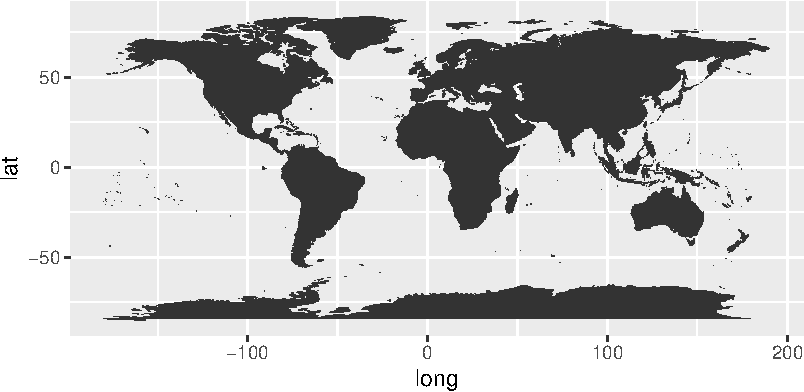
\includegraphics{118_K_maps1_files/figure-pdf/unnamed-chunk-2-1.pdf}

}

\end{figure}

Note:

\begin{itemize}
\tightlist
\item
  \texttt{coord\_quickmap()} adjusts the axes to ensure that longitude
  and latitude are rendered on the same scale. It is very important that
  this aspect ratio is maintained or a country may appear super
  stretched or super squished.
\item
  the \texttt{aes(group=group)} option -- This is SUPER IMPORTANT, so R
  knows which things to connect together
\end{itemize}

\hypertarget{what-about-subsetting-the-data}{%
\subsection{What about subsetting the
data?}\label{what-about-subsetting-the-data}}

\begin{Shaded}
\begin{Highlighting}[]
\CommentTok{\#Subset to get Italy}
\NormalTok{italy }\OtherTok{\textless{}{-}} \FunctionTok{map\_data}\NormalTok{(}\StringTok{"world"}\NormalTok{, }\AttributeTok{region =}\StringTok{"Italy"}\NormalTok{)}

\CommentTok{\#Subset to get USA}
\NormalTok{usa }\OtherTok{\textless{}{-}} \FunctionTok{map\_data}\NormalTok{(}\StringTok{"world"}\NormalTok{, }\AttributeTok{region =}\StringTok{"USA"}\NormalTok{)}
\end{Highlighting}
\end{Shaded}

\hypertarget{what-if-aspect-ratio-is-not-maintained}{%
\subsection{What if aspect ratio is not
maintained?}\label{what-if-aspect-ratio-is-not-maintained}}

\begin{Shaded}
\begin{Highlighting}[]
\CommentTok{\# ASPECT RATIO NOT MAINTAINED}
\FunctionTok{ggplot}\NormalTok{(italy, }\FunctionTok{aes}\NormalTok{(long, lat)) }\SpecialCharTok{+} 
  \FunctionTok{geom\_polygon}\NormalTok{(}\FunctionTok{aes}\NormalTok{(}\AttributeTok{group=}\NormalTok{group)) }\SpecialCharTok{+} 
  \FunctionTok{theme\_light}\NormalTok{() }\SpecialCharTok{+}
  \FunctionTok{ggtitle}\NormalTok{(}\StringTok{"Italy {-} Aspect Ratio Not Maintained (not good)"}\NormalTok{)}
\end{Highlighting}
\end{Shaded}

\begin{figure}[H]

{\centering 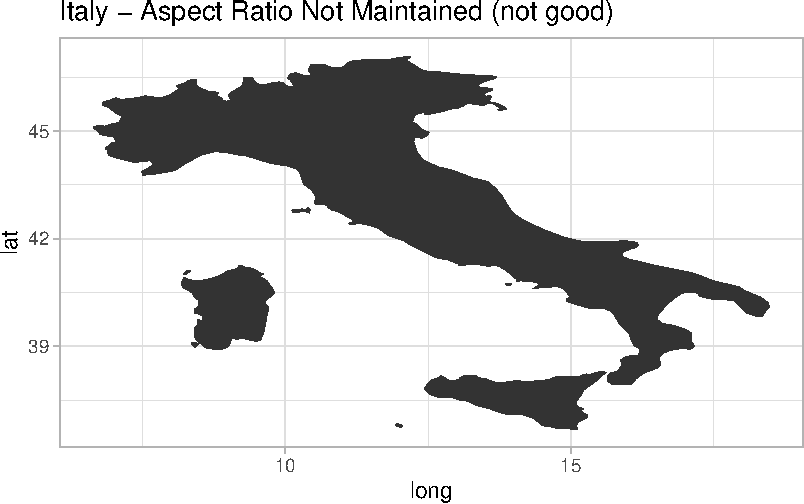
\includegraphics{118_K_maps1_files/figure-pdf/unnamed-chunk-4-1.pdf}

}

\end{figure}

\begin{Shaded}
\begin{Highlighting}[]
\CommentTok{\# ASPECT RATIO MAINTAINED}
\FunctionTok{ggplot}\NormalTok{(italy, }\FunctionTok{aes}\NormalTok{(long, lat)) }\SpecialCharTok{+} 
  \FunctionTok{geom\_polygon}\NormalTok{(}\FunctionTok{aes}\NormalTok{(}\AttributeTok{group=}\NormalTok{group)) }\SpecialCharTok{+} 
  \FunctionTok{coord\_quickmap}\NormalTok{()  }\SpecialCharTok{+}
  \FunctionTok{theme\_light}\NormalTok{() }\SpecialCharTok{+}
  \FunctionTok{ggtitle}\NormalTok{(}\StringTok{"Italy {-} Aspect Ratio Maintained (better)"}\NormalTok{)}
\end{Highlighting}
\end{Shaded}

\begin{figure}[H]

{\centering 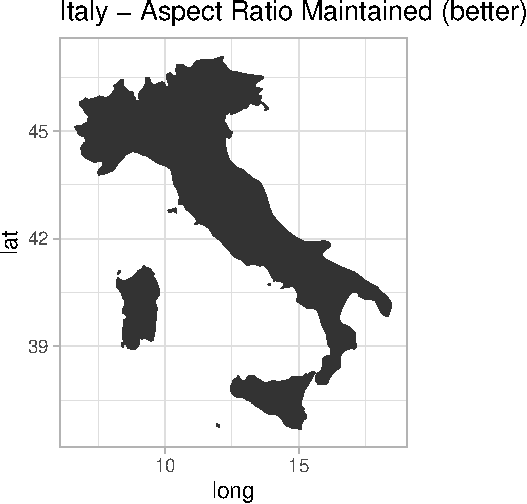
\includegraphics{118_K_maps1_files/figure-pdf/unnamed-chunk-5-1.pdf}

}

\end{figure}

\hypertarget{usa-with-states}{%
\subsection{USA with states}\label{usa-with-states}}

\begin{Shaded}
\begin{Highlighting}[]
\CommentTok{\#Load Data from maps}
\NormalTok{usa\_states }\OtherTok{\textless{}{-}} \FunctionTok{map\_data}\NormalTok{(}\StringTok{"state"}\NormalTok{)}

\CommentTok{\#Plot of USA with state borders}
\FunctionTok{ggplot}\NormalTok{(usa\_states, }\FunctionTok{aes}\NormalTok{(long, lat)) }\SpecialCharTok{+}
\FunctionTok{geom\_polygon}\NormalTok{(}\FunctionTok{aes}\NormalTok{(}\AttributeTok{group=}\NormalTok{group)) }\SpecialCharTok{+}
\FunctionTok{coord\_quickmap}\NormalTok{()}
\end{Highlighting}
\end{Shaded}

\begin{figure}[H]

{\centering 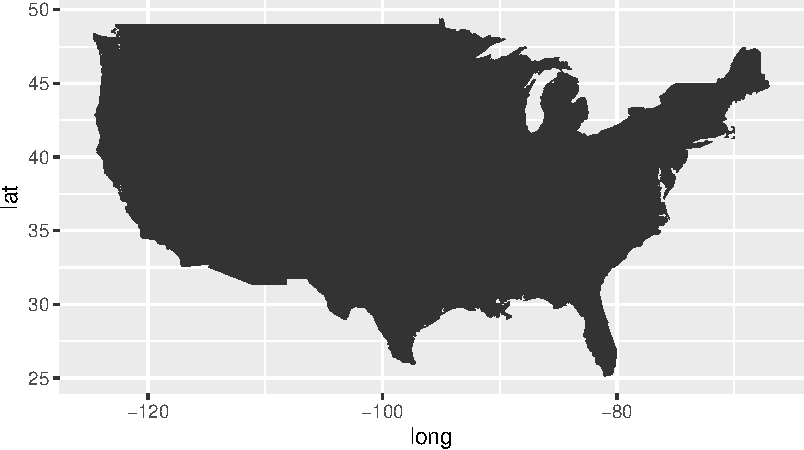
\includegraphics{118_K_maps1_files/figure-pdf/unnamed-chunk-6-1.pdf}

}

\end{figure}

\hypertarget{how-to-customize-colors}{%
\subsection{How to customize colors?}\label{how-to-customize-colors}}

\begin{Shaded}
\begin{Highlighting}[]
\FunctionTok{ggplot}\NormalTok{(usa\_states, }\FunctionTok{aes}\NormalTok{(long, lat)) }\SpecialCharTok{+}
\FunctionTok{geom\_polygon}\NormalTok{(}\FunctionTok{aes}\NormalTok{(}\AttributeTok{group=}\NormalTok{group), }\AttributeTok{fill =}\StringTok{"\#75816b"}\NormalTok{, }\AttributeTok{color =}\StringTok{"\#292c26"}\NormalTok{) }\SpecialCharTok{+}
\FunctionTok{coord\_quickmap}\NormalTok{() }\SpecialCharTok{+}
\FunctionTok{theme\_light}\NormalTok{()}
\end{Highlighting}
\end{Shaded}

\begin{figure}[H]

{\centering 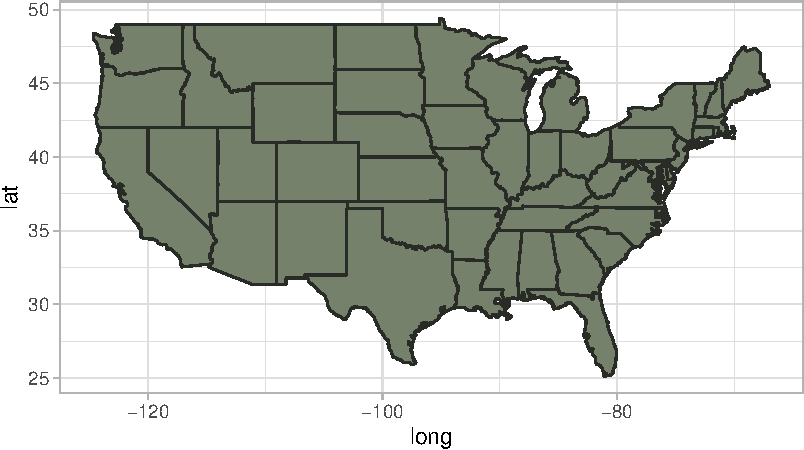
\includegraphics{118_K_maps1_files/figure-pdf/unnamed-chunk-7-1.pdf}

}

\end{figure}

\hypertarget{using-the-sf-package}{%
\section{\texorpdfstring{Using the \texttt{sf}
package}{Using the sf package}}\label{using-the-sf-package}}

There are a few limitations to the approach outlined above, not least of
which is the fact that the simple ``longitude-latitude'' data format is
not typically used in real world mapping. Vector data for maps are
typically encoded using the ``simple features'' standard produced by the
Open Geospatial Consortium. The
\href{https://r-spatial.github.io/sf/}{\texttt{sf}} package developed by
Edzer Pebesma provides an excellent toolset for working with such data,
and the \texttt{geom\_sf()} and \texttt{coord\_sf()} functions in
ggplot2 are designed to work together with the \texttt{sf} package.

\begin{figure}

{\centering \includegraphics{https://user-images.githubusercontent.com/520851/50280460-e35c1880-044c-11e9-9ed7-cc46754e49db.jpg}

}

\caption{Artwork by @allisonhorst}

\end{figure}

\begin{Shaded}
\begin{Highlighting}[]
\CommentTok{\#LOAD PACKAGES}
\CommentTok{\#install.packages("sf") {-} note some students are getting a pop{-}up when they install the sf package for the first time. Select the "no" option when it pops up in your console. }
\FunctionTok{library}\NormalTok{(sf)}

\CommentTok{\#some students are needing into install the rgeos package seperately as well}
\CommentTok{\#library(rgeos)}
\end{Highlighting}
\end{Shaded}

For our first example, we will be working with a dataset of North
Carolina that is built in to the \texttt{sf} package.

\begin{Shaded}
\begin{Highlighting}[]
\FunctionTok{demo}\NormalTok{(nc, }\AttributeTok{ask =} \ConstantTok{FALSE}\NormalTok{, }\AttributeTok{echo =} \ConstantTok{FALSE}\NormalTok{)}
\end{Highlighting}
\end{Shaded}

You should notice that the \texttt{nc} dataset is now saved in your R
environment. This dataset contains information about Sudden Infant Death
Syndrome (SIDS) for North Carolina counties, over two time periods
(1974-78 and 1979-84). Let's take a look at that dataset.

Each row represents a county in North Carolina. This data frame contains
the following columns:

\begin{itemize}
\tightlist
\item
  \texttt{AREA} County polygon areas in degree units
\item
  \texttt{PERIMETER} County polygon perimeters in degree units
\item
  \texttt{CNTY\_} Internal county ID
\item
  \texttt{NAME} County names
\item
  \texttt{FIPS} County ID
\item
  \texttt{FIPSNO} County ID
\item
  \texttt{CRESS\_ID} Cressie papers ID
\item
  \texttt{BIR74} births, 1974-78
\item
  \texttt{SID74} SID deaths, 1974-78
\item
  \texttt{NWBIR74} non-white births, 1974-78
\item
  \texttt{BIR79} births, 1979-84
\item
  \texttt{SID79} SID deaths, 1979-84
\item
  \texttt{NWBIR79} non-white births, 1979-84
\item
  \texttt{geom} information needed to plot the map for each county
\end{itemize}

Let's begin by simply plotting the map:

\begin{Shaded}
\begin{Highlighting}[]
\NormalTok{nc }\SpecialCharTok{\%\textgreater{}\%}
  \FunctionTok{ggplot}\NormalTok{() }\SpecialCharTok{+}
  \FunctionTok{geom\_sf}\NormalTok{()}
\end{Highlighting}
\end{Shaded}

\begin{figure}[H]

{\centering 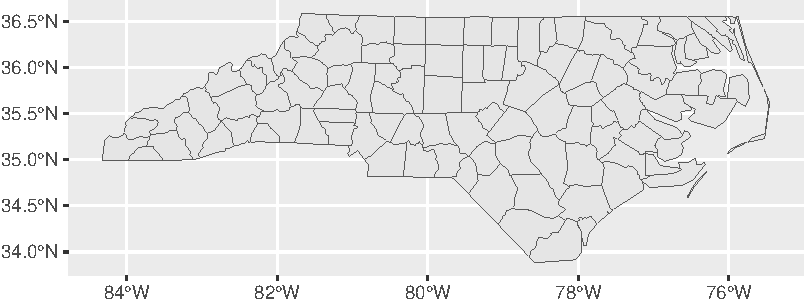
\includegraphics{118_K_maps1_files/figure-pdf/unnamed-chunk-10-1.pdf}

}

\end{figure}

Let's pretty it up:

\begin{Shaded}
\begin{Highlighting}[]
\NormalTok{nc }\SpecialCharTok{\%\textgreater{}\%}
  \FunctionTok{ggplot}\NormalTok{() }\SpecialCharTok{+}
  \FunctionTok{geom\_sf}\NormalTok{(}\AttributeTok{col=}\StringTok{"black"}\NormalTok{, }\AttributeTok{fill=}\StringTok{"darkgrey"}\NormalTok{) }\SpecialCharTok{+}
  \FunctionTok{theme\_light}\NormalTok{() }\SpecialCharTok{+}
  \FunctionTok{ggtitle}\NormalTok{(}\StringTok{"North Carolina Counties"}\NormalTok{)}
\end{Highlighting}
\end{Shaded}

\begin{figure}[H]

{\centering 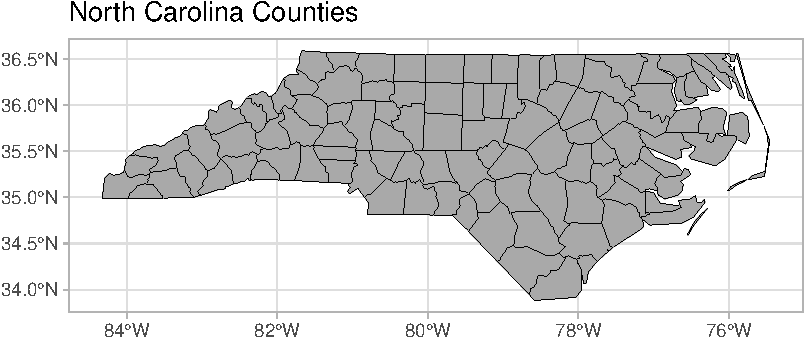
\includegraphics{118_K_maps1_files/figure-pdf/unnamed-chunk-11-1.pdf}

}

\end{figure}

\hypertarget{cloropleth-maps}{%
\section{Cloropleth maps}\label{cloropleth-maps}}

Suppose we want to shade each of these counties, based on the number of
births in 1974.

This is called a ``cloropleth'' map (a map that uses differences in
shading, coloring, or the placing of symbols within predefined areas to
indicate the average values of a property or quantity in those areas).

\begin{Shaded}
\begin{Highlighting}[]
\NormalTok{nc }\SpecialCharTok{\%\textgreater{}\%}
  \FunctionTok{ggplot}\NormalTok{() }\SpecialCharTok{+}
  \FunctionTok{geom\_sf}\NormalTok{( }\FunctionTok{aes}\NormalTok{(}\AttributeTok{fill =}\NormalTok{ BIR74), }\AttributeTok{col =}\StringTok{"black"}\NormalTok{) }\SpecialCharTok{+}
  \FunctionTok{theme\_light}\NormalTok{()}\SpecialCharTok{+}
  \FunctionTok{ggtitle}\NormalTok{(}\StringTok{"North Carolina, Birth Rates in 1974"}\NormalTok{)}
\end{Highlighting}
\end{Shaded}

\begin{figure}[H]

{\centering 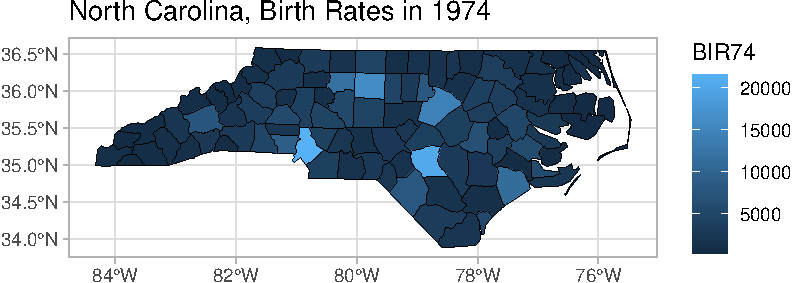
\includegraphics{118_K_maps1_files/figure-pdf/unnamed-chunk-12-1.pdf}

}

\end{figure}

Here are some options to customize the plot that you might be interested
in:

\hypertarget{using-rcolorbrewer-palette}{%
\subsubsection{Using RColorBrewer
palette}\label{using-rcolorbrewer-palette}}

\begin{Shaded}
\begin{Highlighting}[]
\FunctionTok{library}\NormalTok{(RColorBrewer)}

\NormalTok{nc }\SpecialCharTok{\%\textgreater{}\%}
  \FunctionTok{ggplot}\NormalTok{() }\SpecialCharTok{+}
  \FunctionTok{geom\_sf}\NormalTok{(}\FunctionTok{aes}\NormalTok{(}\AttributeTok{fill =}\NormalTok{ BIR74)) }\SpecialCharTok{+}
  \FunctionTok{ggtitle}\NormalTok{(}\StringTok{"North Carolina, Birth Rates in 1974"}\NormalTok{) }\SpecialCharTok{+}
  \FunctionTok{scale\_fill\_gradientn}\NormalTok{(}\AttributeTok{colors =} \FunctionTok{brewer.pal}\NormalTok{(}\DecValTok{8}\NormalTok{,}\StringTok{"Spectral"}\NormalTok{) ) }\SpecialCharTok{+} \CommentTok{\#customize colors}
  \FunctionTok{theme\_light}\NormalTok{()}
\end{Highlighting}
\end{Shaded}

\begin{figure}[H]

{\centering 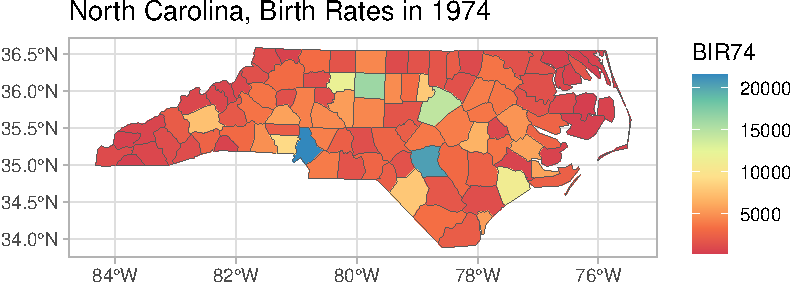
\includegraphics{118_K_maps1_files/figure-pdf/unnamed-chunk-13-1.pdf}

}

\end{figure}

\hypertarget{using-part-of-a-rcolorbrewer-palette}{%
\subsubsection{Using part of a RColorBrewer
palette}\label{using-part-of-a-rcolorbrewer-palette}}

\begin{Shaded}
\begin{Highlighting}[]
\NormalTok{nc }\SpecialCharTok{\%\textgreater{}\%}
  \FunctionTok{ggplot}\NormalTok{() }\SpecialCharTok{+}
  \FunctionTok{geom\_sf}\NormalTok{(}\FunctionTok{aes}\NormalTok{(}\AttributeTok{fill =}\NormalTok{ BIR74)) }\SpecialCharTok{+}
  \FunctionTok{ggtitle}\NormalTok{(}\StringTok{"North Carolina, Birth Rates in 1974"}\NormalTok{) }\SpecialCharTok{+}
  \FunctionTok{scale\_fill\_gradientn}\NormalTok{(}\AttributeTok{colors =} \FunctionTok{brewer.pal}\NormalTok{(}\DecValTok{11}\NormalTok{,}\StringTok{"Spectral"}\NormalTok{)[}\DecValTok{5}\SpecialCharTok{:}\DecValTok{11}\NormalTok{] ) }\SpecialCharTok{+} \CommentTok{\#customize colors}
  \FunctionTok{theme\_light}\NormalTok{()}
\end{Highlighting}
\end{Shaded}

\begin{figure}[H]

{\centering 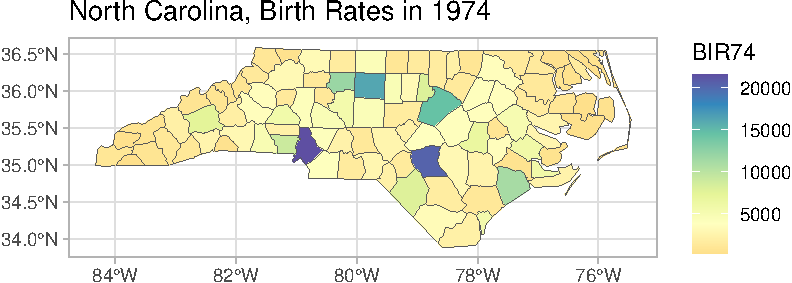
\includegraphics{118_K_maps1_files/figure-pdf/unnamed-chunk-14-1.pdf}

}

\end{figure}

\hypertarget{building-your-own-color-palette-using-scale_fill_gradientn}{%
\subsubsection{\texorpdfstring{Building your own color palette using
\texttt{scale\_fill\_gradientn}}{Building your own color palette using scale\_fill\_gradientn}}\label{building-your-own-color-palette-using-scale_fill_gradientn}}

\begin{Shaded}
\begin{Highlighting}[]
\NormalTok{nc }\SpecialCharTok{\%\textgreater{}\%}
  \FunctionTok{ggplot}\NormalTok{() }\SpecialCharTok{+}
  \FunctionTok{geom\_sf}\NormalTok{(}\FunctionTok{aes}\NormalTok{(}\AttributeTok{fill =}\NormalTok{ BIR74)) }\SpecialCharTok{+}
  \FunctionTok{ggtitle}\NormalTok{(}\StringTok{"North Carolina, Birth Rates in 1974"}\NormalTok{) }\SpecialCharTok{+}
  \FunctionTok{scale\_fill\_gradientn}\NormalTok{(}\AttributeTok{colors =} \FunctionTok{c}\NormalTok{(}\StringTok{"yellow"}\NormalTok{,}\StringTok{"orange"}\NormalTok{,}\StringTok{"red"}\NormalTok{))}
\end{Highlighting}
\end{Shaded}

\begin{figure}[H]

{\centering 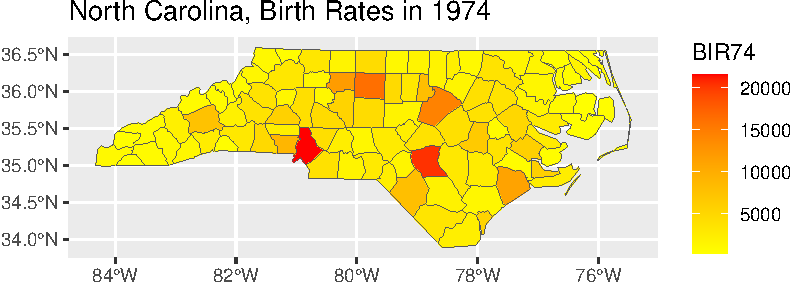
\includegraphics{118_K_maps1_files/figure-pdf/unnamed-chunk-15-1.pdf}

}

\end{figure}

A note about customizing colors:

\begin{itemize}
\tightlist
\item
  you should use a color scheme that is sequential (has order to it),
  when you are displaying continuous data
\item
  you should use a color scheme that is categorical, when your data is
  in categories and isn't ordered you should use a color scheme that is
  diverging, when want to put emphasis on two extremes and mid-range.
  For example, you might use a diverging palette from red to blue for
  political party affiliation in the US.
\item
  pay attention to your map being color blind friendly (\texttt{RdYlGr}
  is the worst\ldots)
\item
  as a general rule, try not to use blue to represent a land mass (let's
  reserve that for bodies of water)
\end{itemize}

\hypertarget{adding-labels}{%
\subsection{Adding labels}\label{adding-labels}}

\begin{Shaded}
\begin{Highlighting}[]
\FunctionTok{ggplot}\NormalTok{(nc) }\SpecialCharTok{+} 
  \FunctionTok{geom\_sf}\NormalTok{() }\SpecialCharTok{+} 
  \FunctionTok{aes}\NormalTok{(}\AttributeTok{fill =}\NormalTok{ BIR74) }\SpecialCharTok{+}
  \FunctionTok{ggtitle}\NormalTok{(}\StringTok{"North Carolina, Birth Rates in 1974"}\NormalTok{) }\SpecialCharTok{+}
  \FunctionTok{scale\_fill\_gradientn}\NormalTok{(}\AttributeTok{colors =} \FunctionTok{brewer.pal}\NormalTok{(}\DecValTok{8}\NormalTok{, }\StringTok{"Spectral"}\NormalTok{) ) }\SpecialCharTok{+}  \CommentTok{\#customize colors}
  \FunctionTok{theme\_light}\NormalTok{() }\SpecialCharTok{+}
  \FunctionTok{geom\_sf\_text}\NormalTok{(}\AttributeTok{data =}\NormalTok{ nc[nc}\SpecialCharTok{$}\NormalTok{BIR74 }\SpecialCharTok{\textgreater{}}\DecValTok{15000}\NormalTok{,], }\FunctionTok{aes}\NormalTok{(}\AttributeTok{label =}\NormalTok{ NAME), }\AttributeTok{fontface=}\StringTok{"bold"}\NormalTok{)}
\end{Highlighting}
\end{Shaded}

\begin{figure}[H]

{\centering 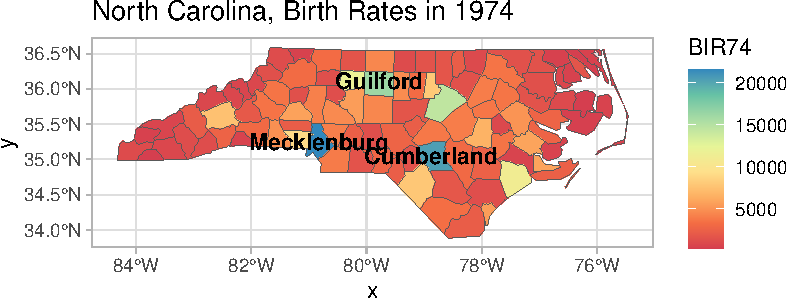
\includegraphics{118_K_maps1_files/figure-pdf/unnamed-chunk-16-1.pdf}

}

\end{figure}

\hypertarget{sf-cheatsheet}{%
\section{\texorpdfstring{\texttt{sf}
cheatsheet}{sf cheatsheet}}\label{sf-cheatsheet}}

\href{https://github.com/rstudio/cheatsheets/blob/a045e18875cde4c9cf9c7f5f8bee71b4c8c2a2b7/sf.pdf}{\texttt{sf}
cheatsheet}



\end{document}
